\documentclass{article}
\newcommand\hmmax{0}
\newcommand\bmmax{0}
\usepackage{booktabs}

%% Language and font encodings
\usepackage[english]{babel}
\usepackage[utf8x]{inputenc}
\usepackage[T1]{fontenc}
\usepackage{gensymb}
\usepackage{pdfpages}

\usepackage[bitstream-charter]{mathdesign}
\let\circledS\undefined
%% Sets page size and margins
\usepackage[a4paper,top=2cm,bottom=2cm,left=1cm,right=1cm, marginparsep=1cm]{geometry}

%% Useful packages
\usepackage{amsmath}
\usepackage{bm}
\usepackage[makeroom]{cancel}
\usepackage{enumitem}
\usepackage{listings}
\usepackage{multirow}
\usepackage{amssymb}
\usepackage{float}
\usepackage{graphicx}
\usepackage{wrapfig}

\newcommand{\myq}[1]{%
	\vspace{1em}
	\noindent\underline{\emph{Exercise #1}}\vspace{0.25em}\linebreak
}

\DeclareMathAlphabet{\altmathcal}{OMS}{cmsy}{m}{n}

\usepackage[noend]{algpseudocode}
\usepackage{algorithm,algorithmicx}

\newcommand*\Let[2]{\State #1 $\gets$ #2}
\algrenewcommand\algorithmicrequire{}
\algrenewcommand\algorithmicensure{\textbf{Postcondition:}}

\title{\textbf{Reinforcement Learning: An Introduction}\\
\textit{Solutions: Chapter 4}
}
\author{Mrinank Sharma}

\begin{document}
\maketitle

\myq{4.1}
\begin{align}
q_\pi(11, \texttt{down}) = -1 + v_\pi(\texttt{terminal}) = -1. \\
q_\pi(7, \texttt{down}) = -1 + v_\pi(11) = -1 -14 = -15 .
\end{align}  

\myq{4.2: MDP Modifications}
\textbf{Unchanged dynamics from current states}. In this case, the value of these states from these policies is unchanged, we've simply introduced a new state. We can calculate the value of this state using the Bellman equations:
\begin{align}
v_\pi(15) = -1 + \frac{1}{4}[-22 -20 -14 +v_\pi(15)] \Rightarrow v_\pi(15) = -20.
\end{align}
\textbf{Dynamics changed from state $13$}. In general, we'd expect this to change the value of state $13$, which would propagate to all of the other states, meaning that we'd have to recalculate the values. Let's pretend that we were running iterative policy evaluation using the previous value function as our initialisation. Let's update the value for state $13$:
\begin{align}
v_\pi(13) = -1 + \frac{1}{4}[-20 -22 -14 \underbrace{-20}_{\text{Estimate for } v_\pi(15)}] = -20
\end{align}
\textbf{The value of state $13$ hasn't changed!} Therefore, the value of state $15$, and all of the other states also won't change. We've recalculated values without having to solve those annoying equations, which is nice. 

\myq{4.3: Iterative Action-Value Evaluation}
\begin{align}
q_\pi(s, a) &=\mathbb{E}_\pi[G_t | S_t = s, A_t = a] \nonumber \\
&= \mathbb{E}_\pi[R_{t+1} + \gamma G_{t+1} | S_t = s, A_t = a] \nonumber \\
&= \sum_{s' \in \altmathcal{S}, r \in \altmathcal{R}} p(s', r | s, a) [r + \gamma \sum_{a \in \altmathcal{A}(s')} \pi(a' | s')[q_\pi(s', a')]],
\end{align}
which can straightforwardly be turned into an iterative update equation. 

\myq{4.4: Policy Iteration Bug}
If policy is switching between policies which are equally good, both of the policies are optimal. There must be multiple actions in each step which give the same expected optimal return, and the suggested algorithm does not state how to break ties. We should be able to fix this by settling ties in the $\arg\max$ operation, for example, by indexing all of the actions and always choosing the lowest index amongst optimal options. 

\begin{algorithm}[H]
	\caption{Policy Iteration
		\label{alg:policy_eval}}
	\begin{algorithmic}[1]
		\Require{
			\textbf{Initialisation:} initialise $V(s)$ arbitarily for all $s \in \altmathcal{S}$ except that $V(\text{terminal})=0$. Initalise $\pi(s) \in \altmathcal{A}(s)$ arbitrarily for all $s \in \altmathcal{S}$.} 
		\Require{\textbf{Parameters: } $\theta > 0$, a threshold determining accuracy.}
		\Statex
		\Loop: \Comment{Policy Evaluation} \label{alg:policy_iteration:eval_loop}
		\Let{$\Delta$}{0}
		\For{each $s \in \altmathcal{S}$}: 
		\Let{$v$}{$V(s)$}
		\Let{$V(s)$}{$\sum_{a \in \altmathcal{A}(s)} \pi(a|s) \sum_{s' \in \altmathcal{S}, r \in \altmathcal{R}} p(s', r | s, a) [r + \gamma V(s')]$}
		\Let{$\Delta$}{$\max(\Delta, |v - V(s)|)$}
		\EndFor
		\EndLoop\\\textbf{until $\Delta < \theta$}
		\Statex
		\Let{$\texttt{policy-stable}$}{True} \Comment{Policy Improvement}
		\For{each $s \in \altmathcal{S}$}: 
		\Let{\texttt{old-action}}{$\pi(s)$}
		\Let{$\pi(s)$}{$\arg \max_{a \in \altmathcal{A}(s)} \sum_{s' \in \altmathcal{S}, r \in \altmathcal{R}} p(s', r | s, a) [r + \gamma V(s')]$} \Comment{Settle ties by index.}
		\If{\texttt{old-action} $\neq \pi(s)$}: 
		\Let{$\texttt{policy-stable}$}{True}
		\EndIf
		\EndFor
		\If{\texttt{policy-stable}}:
		\State \Return $V \simeq v_*, \pi 
		\simeq \pi* $
		\Else: \State \textbf{ go to} \ref{alg:policy_iteration:eval_loop}
		\EndIf
	\end{algorithmic}
\end{algorithm}

\myq{4.5: Policy Iteration with $q(s, a)$}
I will assume deterministic policies here, using the same bug fix. 
\begin{algorithm}[H]
	\caption{$Q$ Iteration
		\label{alg:q_policy_eval}}
	\begin{algorithmic}[1]
		\Require{
			\textbf{Initialisation:} initialise $Q(a, s)$ arbitarily for all $s \in \altmathcal{S}, a \in \altmathcal{A}$ except that $Q(\text{terminal}, a)=0\quad \forall a$. Initalise $\pi(s) \in \altmathcal{A}(s)$ arbitrarily for all $s \in \altmathcal{S}$.} 
		\Require{\textbf{Parameters: } $\theta > 0$, a threshold determining accuracy.}
		\Statex
		\Loop: \Comment{Policy Evaluation} \label{alg:q_policy_iteration:eval_loop}
		\Let{$\Delta$}{0}
		\For{each $s \in \altmathcal{S}$}: 
			\For{each $a \in \altmathcal{A}(s)$}
		\Let{$q$}{$Q(s, a)$}
		\Let{$Q(s, a)$}{$\sum_{s' \in \altmathcal{S}, r \in \altmathcal{R}} p(s', r | s, a)[r + \gamma Q(s', \pi(s'))]$}
		\Let{$\Delta$}{$\max(\Delta, |q - Q(s, a)|)$}
		\EndFor
		\EndFor
		\EndLoop\\\textbf{until $\Delta < \theta$}
		\Statex
		\Let{$\texttt{policy-stable}$}{True} \Comment{Policy Improvement}
		\For{each $s \in \altmathcal{S}$}: 
		\Let{\texttt{old-action}}{$\pi(s)$}
		\Let{$\pi(s)$}{$\arg \max_{a \in \altmathcal{A}(s)} Q(s, a)$} \Comment{Settle ties by index.}
		\If{\texttt{old-action} $\neq \pi(s)$}: 
		\Let{$\texttt{policy-stable}$}{True}
		\EndIf
		\EndFor
		\If{\texttt{policy-stable}}:
		\State \Return $Q \simeq q_*, \pi 
		\simeq \pi* $
		\Else: \State \textbf{ go to} \ref{alg:q_policy_iteration:eval_loop}
		\EndIf
	\end{algorithmic}
\end{algorithm}

\myq{4.6: $\epsilon$-soft policies}
Let's restrict ourself to determinstic + $\epsilon$-soft policies. i.e.,
\begin{align}
\pi(a | s) = \begin{cases}
1 - \frac{|\altmathcal{A}(s)| - 1 }{|\altmathcal{A}(s)|}\epsilon, \quad &a = \pi_d(s) \\
\frac{\epsilon}{\altmathcal{A}(s)}, &\text{otherwise}
\end{cases},
\end{align}
where $\pi_d$ is now effectively the determinstic part of the policy. Now, we make the following changes:
\begin{enumerate}[noitemsep]
	\item No change to the initialise of the algorithm. 
	\item Update the value of the policy by adding a marginalisation step over the possible actions to be selected. 
	\item In policy improvement, update only the determinstic part of the policy, but using the value of the soft policy to perform the updates. 
\end{enumerate}

\textbf{Note: not fully clear to me that considering this form is policy is sufficient. There are many stochastic policies which we could add a soft part to.}

\myq{4.7: Policy Iteration}
Note that we cheated by truncating the poisson distributions (as in the Github replication of the original figure) and also returned a constant number of cars (also as in the reproduction) to make the code run faster. Relevant code is on the Github repo. The replication from the book is found in Fig.~\ref{fig:original_sol}.

The solution to the modified problem can be seen in Fig.~\ref{fig:modified_sol}. The shape is pretty wacky. As expected, we play $1$ quite frequently now because it is free for us to move a car from location $1$ to $2$ (and it it also often makes sense because of the demands are these places). 

\begin{figure}
	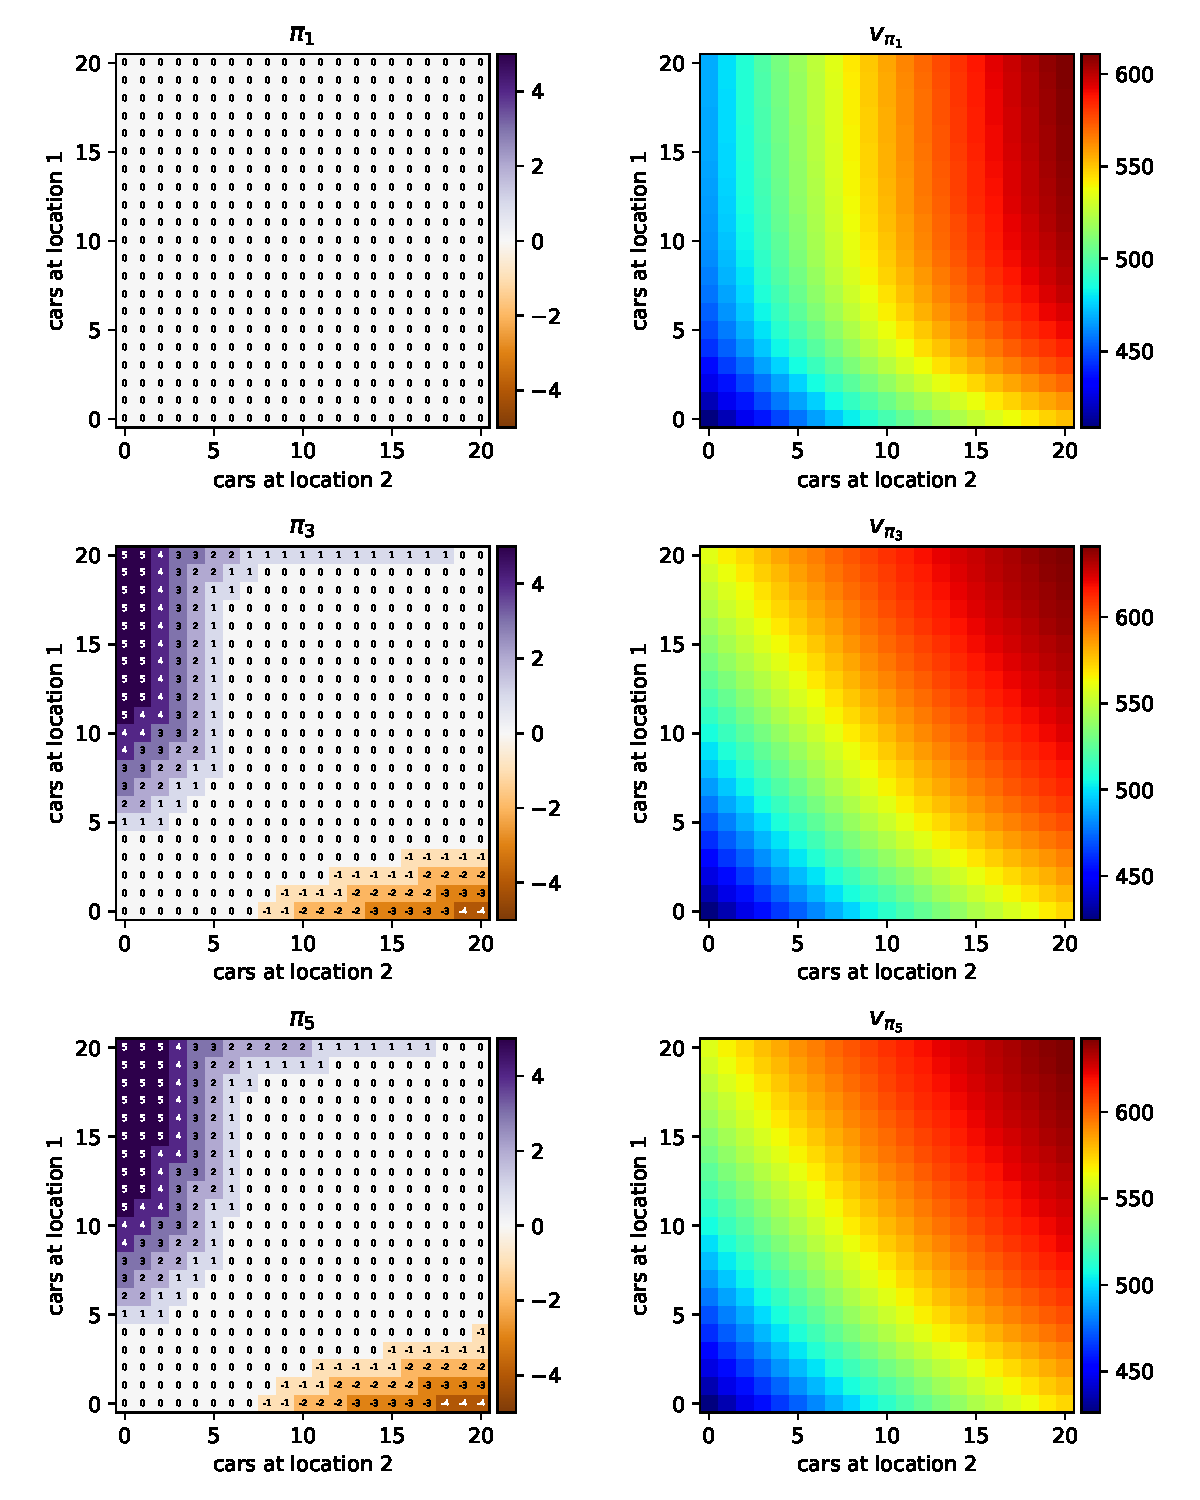
\includegraphics[width=\textwidth]{original}
	\centering
	\caption{\label{fig:original_sol} Replication of Fig. 4.2}
\end{figure}

\begin{figure}
	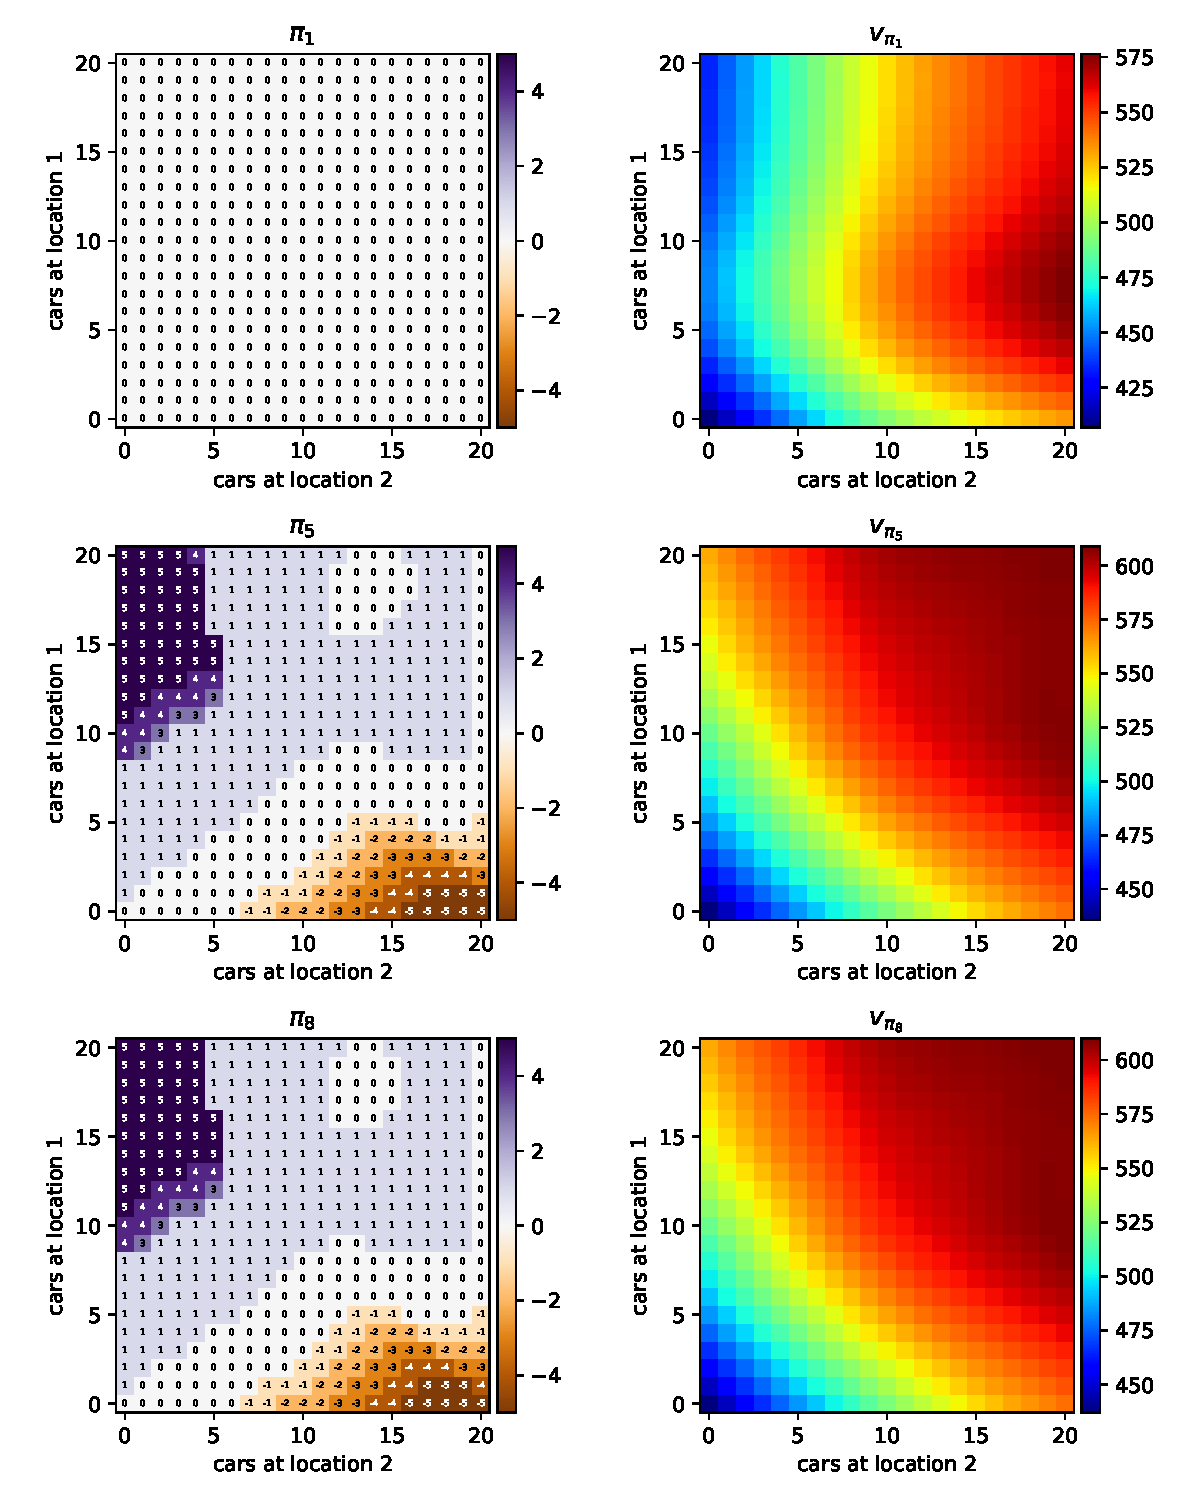
\includegraphics[width=\textwidth]{modified}
	\centering
	\caption{\label{fig:modified_sol} Modified Problem Solution}
\end{figure} 

State and action space isn't that big here and still dynamic programming was very very slow! We had to perform truncation and an incorrect approximation to get this solution. This shows the limitation of this method, as wonderful as it is. 

\myq{4.8: Gambler's Problem I}
I'm a bit confused about this problem! It definitely seems super strange to me. Here are some thoughts:
\begin{itemize}[noitemsep]
	\item The coin is biased \textit{against} us. Paths which require shorter succesful flips are much more likely to happen, and so we should favour them. 
	\item Gambling as much as possible, but not more than needed seems to be good. This always give a (minimum of) $40\%$ of winning. Indeed, from $50$ dollars , this is what the optimal strategy does.
	\item It seems super strange to me that betting $50$ dollars is optimal at $50$, but if you have one more dollar, you should bet only $1$? I would have thought betting $49$ dollars in this case would be best. 
\end{itemize}
I looked a bit online and it seems that families of optimal policies are basically the bets which could take us to the peaks of the policy graph e.g., from $51$ bets could be $1, 24$ or $49$. But honestly, I don't really see why. 

Since the coin is against us, if we bet on making lots of conservative bets, in expected value, the value will keep going down and down. 
\begin{align}
\mathbb{E}[c_{t+1}] &= c_t - b + p\cdot 2b = c_t -b (1 - 2p)  
\end{align}
So in general, we ought to minimise the expected number of flips to success. If we made loads of small bets, basically the law of large numbers would mean that eventually we'd definitely lose all of our money. But, if we make small numbers of bets, we basically are far more likely to \emph{get lucky}, so in general, this is what we should do. Its interesting that this is \textbf{not} what the strategy does! It doesn't bet it all when capital is greater than fifty, even though it could. 

See. Fig.~\ref{fig:reprod} for a reproduction. This shows that there are indeed multiple optimal moves. The strategy of always betting the most you can works well. Its funny that move of $0$ always seems to be optimal too, showing that you can never increase your chance of winning on average. The strategy seems to head to the attractor points.   

I think there is a lot more that could be said for this problem. 

\textcolor{red}{I don't think that this is particularly insightful. If you have anything better, please contact me!}

\begin{figure}
	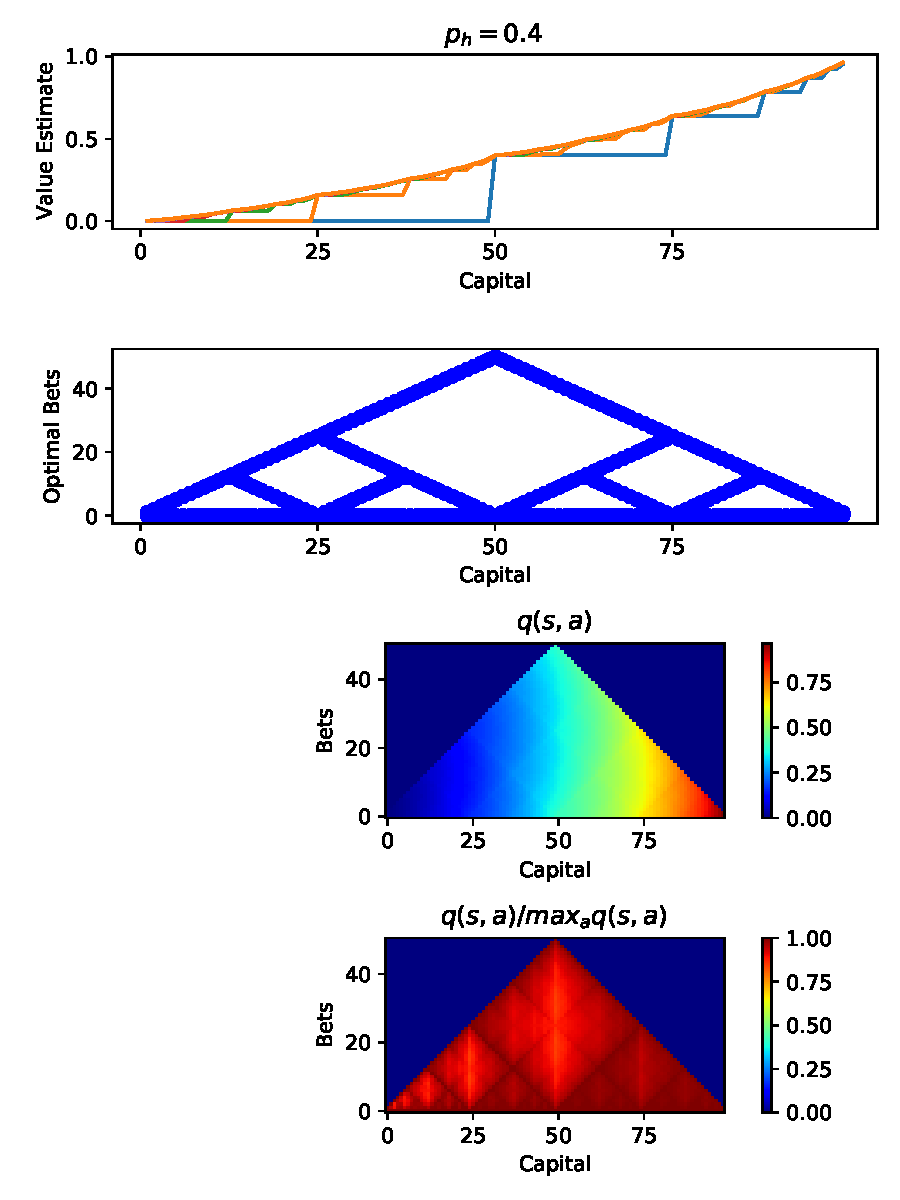
\includegraphics[width=\textwidth]{reprod}
	\centering
	\caption{\label{fig:reprod} Reproduction of Gamblers Problem}
\end{figure} 

\myq{4.9: Programming the Gamblers Problem}
Please see Figures \ref{fig:more_unfair}, \ref{fig:more_unfair}, \ref{fig:less_unfair_more_runs}, \ref{fig:less_unfair_even_more_runs} for results.

The solution is not stable when the coin is biased to give the player the advantage. Note that the solutions that we do get however play much more conservatively - we want to play many games now, because, on average, we expect to win. 

When the coin is even more biased against us, we get the same strategy with less value, which is not surprising. 

Note that we haven't employed discounting here (i.e., we don't care how long we are playing for). If we did, I think the solution would be stable (though I haven't tried it). 

\begin{figure}
	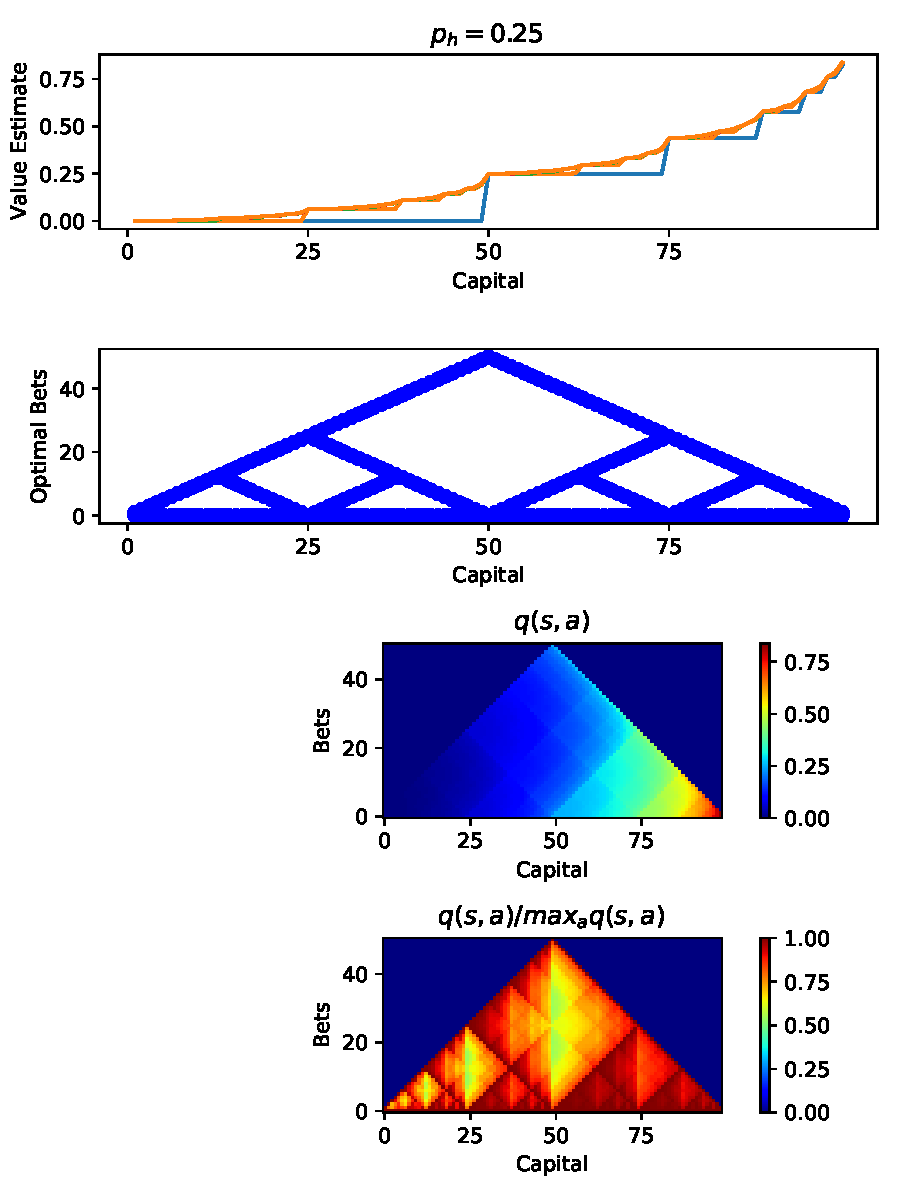
\includegraphics[width=\textwidth]{more_unfair}
	\centering
	\caption{\label{fig:more_unfair} less chance of winning}
\end{figure} 

\begin{figure}
	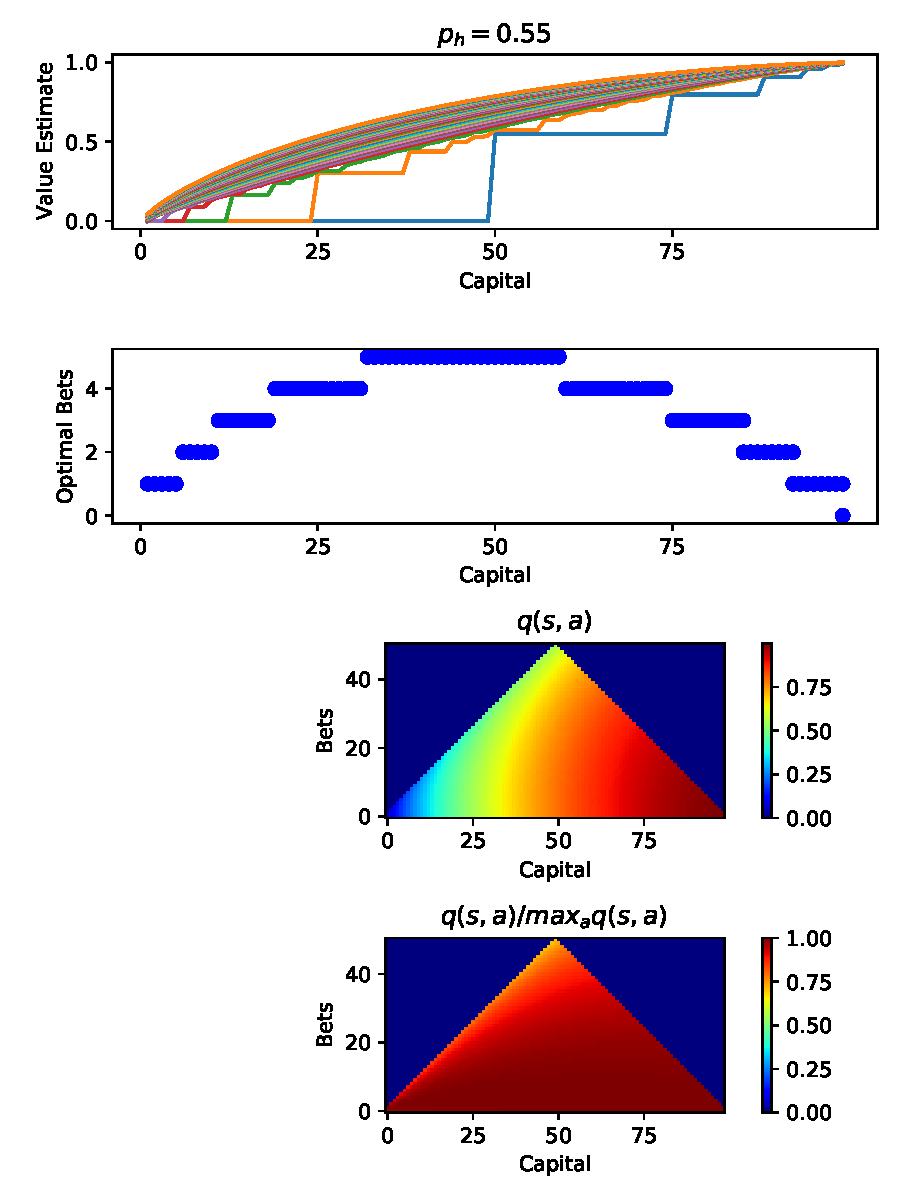
\includegraphics[width=\textwidth]{less_unfair}
	\centering
	\caption{\label{fig:less_unfair}better chance of winning}
\end{figure} 

\begin{figure}
	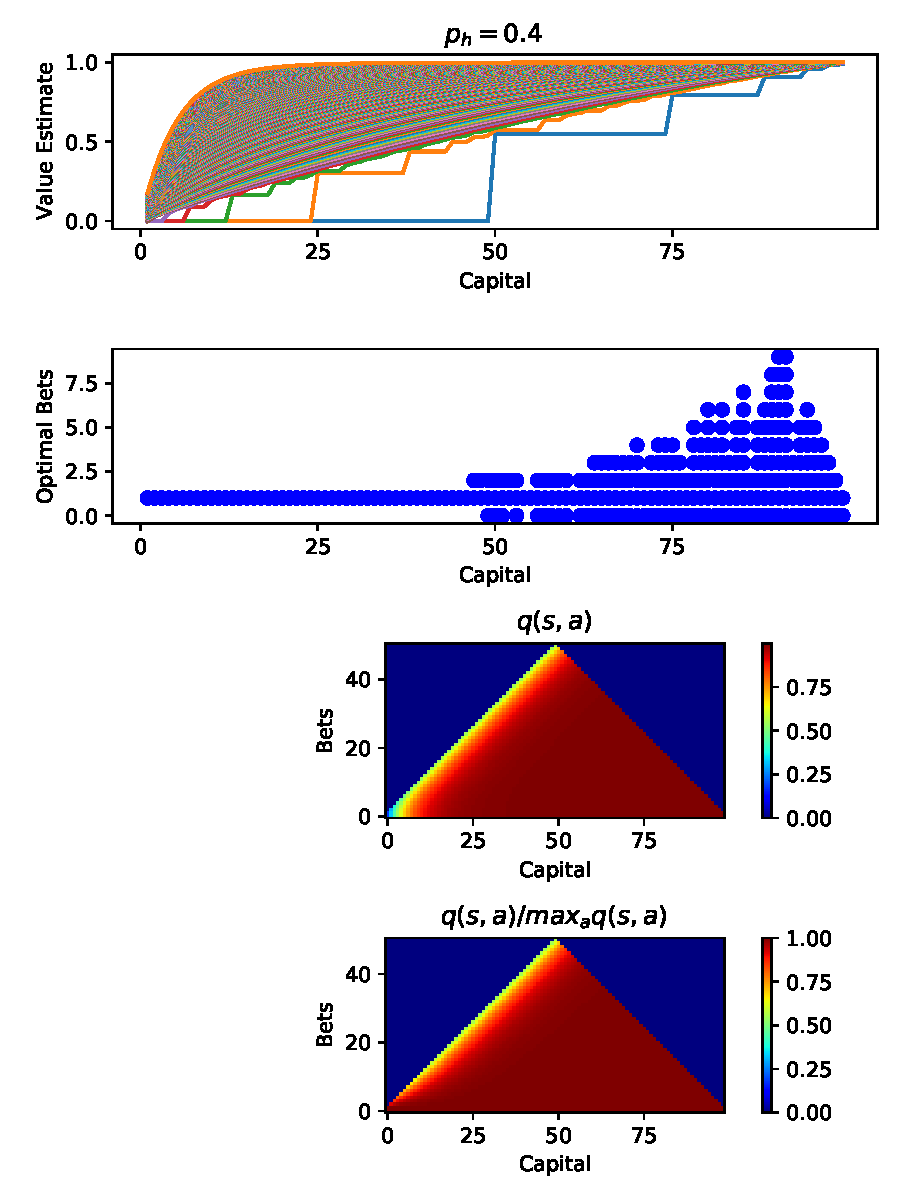
\includegraphics[width=\textwidth]{less_unfair_more_runs}
	\centering
	\caption{\label{fig:less_unfair_more_runs}better chance of winning, $512$ steps of value iteration}
\end{figure} 

\begin{figure}
	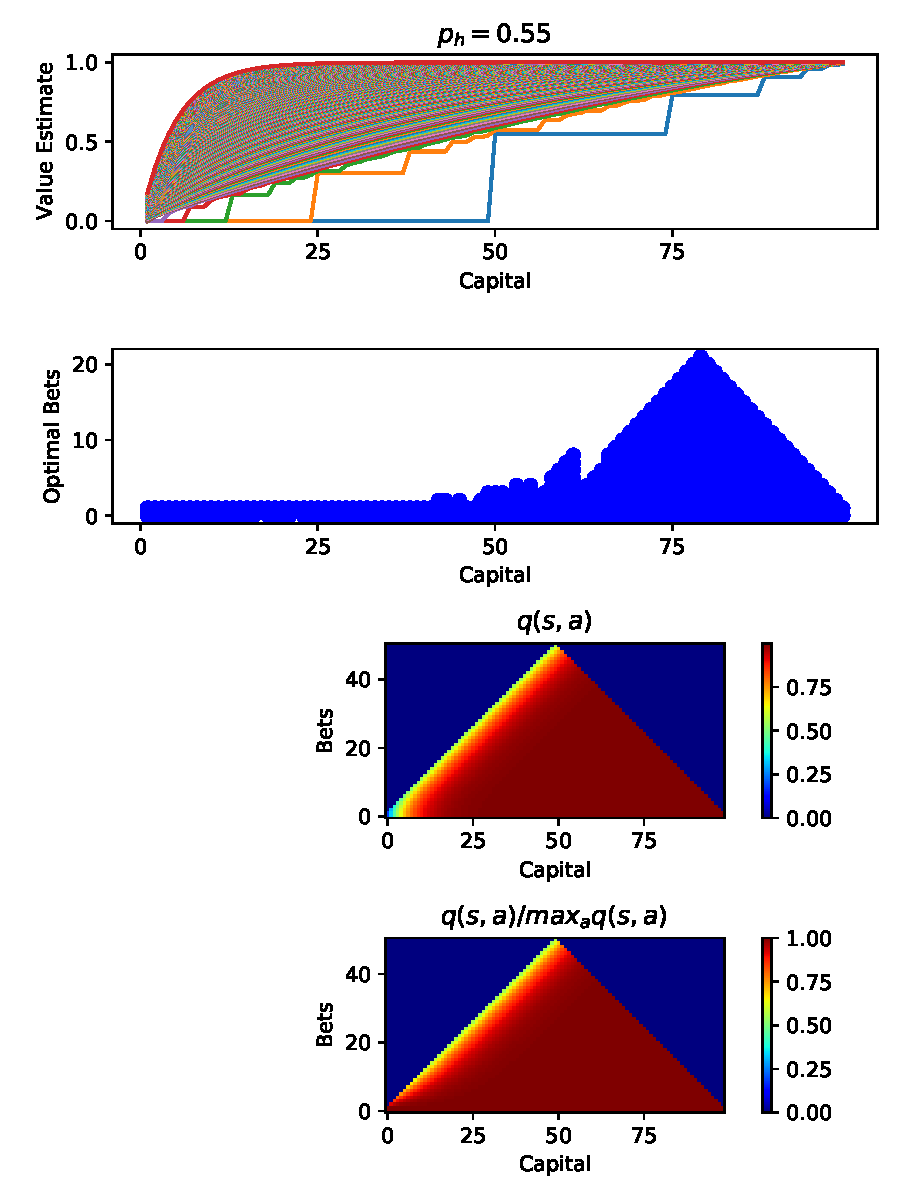
\includegraphics[width=\textwidth]{less_unfair_even_more_runs}
	\centering
	\caption{\label{fig:less_unfair_even_more_runs}better chance of winning, $1024$ steps of value iteration}
\end{figure} 

\myq{4.10: $Q$-Value Iteration}
\begin{align}
q_{k+1}(s, a) = \sum_{s' \in \altmathcal{S}, r \in \altmathcal{R}} p(s', r | s, a)[r + \gamma \max_{a' \in \altmathcal{A}(s')} q_k(s', a') ],
\end{align}
which is very similar to $Q$-Learning (but of course, here we know the MDP we are in). 



\end{document}